\documentclass[rmp,10pt,onecolumn,fleqn,notitlepage]{revtex4-1}

\usepackage{graphicx}
\usepackage{color}
\usepackage{latexsym,amsmath}
\usepackage{physics}
\usepackage{tabularx}
\usepackage{float}
\usepackage{siunitx}
\usepackage{amssymb}

% Listing packages
\usepackage{xcolor}
\usepackage{listings}
\usepackage{framed}
\usepackage{inconsolata} % To change the listing font

% URL package and setting
\definecolor{linkcolor}{rgb}{0,0,0.65} %hyperlink
\usepackage[pdftex,colorlinks=true, pdfstartview=FitV, linkcolor= linkcolor, citecolor= linkcolor, urlcolor= linkcolor, hyperindex=true,hyperfigures=true]{hyperref} %hyperlink%

\usepackage{fancyhdr} % To change page setting

% PAGE SETTING
\pagestyle{fancyplain}
\fancyhf{}
\fancyfoot[R]{\thepage}
\fancyfoot[L]{\today}
\fancyhead[L]{\textbf{Week 7 Report, Quantum Information and Computing (2020)}}
\fancyhead[R]{\textbf{Alice Pagano}}
\renewcommand{\headrulewidth}{0.1pt}
\renewcommand{\footrulewidth}{0.1pt}

% LISTING SETTINGS
\definecolor{cadmiumred}{rgb}{0.89, 0.0, 0.13}
\definecolor{codegray}{rgb}{0.5,0.5,0.5}
\definecolor{commentcolour}{rgb}{0.43,0.63,0.65}
\definecolor{darkgreen}{rgb}{0.0, 0.5, 0.0}

\lstdefinestyle{Fortran}{language=Fortran,
    backgroundcolor=\color{white},
    commentstyle=\color{commentcolour},
    keywordstyle=\bfseries\color{cadmiumred},
    numberstyle=\tiny\color{codegray},
    stringstyle=\color{darkgreen},
    basicstyle=\ttfamily\footnotesize,
    breakatwhitespace=false,
    breaklines=true,
    captionpos=b,
    keepspaces=true,
    numbers=left,
    numbersep=5pt,
    showspaces=false,
    showstringspaces=false,
    showtabs=false,
    tabsize=2,
    frame=single,
    framexleftmargin=11pt,
    %rulecolor=\color{cadmiumred}
}
%\lstset{style=Fortran}

\lstdefinestyle{Gnuplot}{
    backgroundcolor=\color{white},
    commentstyle=\color{commentcolour},
    basicstyle=\ttfamily\footnotesize,
    breakatwhitespace=false,
    breaklines=true,
    captionpos=b,
    keepspaces=true,
    showspaces=false,
    showstringspaces=false,
    showtabs=false,
    tabsize=2
}

\lstdefinestyle{Python}{language=Python,
    backgroundcolor=\color{white},
    commentstyle=\color{commentcolour},
    keywordstyle=\color{darkgreen},
    numberstyle=\tiny\color{codegray},
    stringstyle=\color{cadmiumred},
    basicstyle=\ttfamily\footnotesize,
    breakatwhitespace=false,
    breaklines=true,
    captionpos=b,
    keepspaces=true,
    numbers=left,
    numbersep=5pt,
    showspaces=false,
    showstringspaces=false,
    showtabs=false,
    tabsize=2,
    frame=single,
    framexleftmargin=11pt
}

% BIBLIOGRAPHY FILE AND SETTING
\begin{filecontents*}{\jobname.bib}
    @article{cite1,
      title={Error handling in Fortran 2003},
      author={Koen Poppe and Ronald Cools and Bart Vandewoestyne},
      journal={ACM Sigplan Fortran Forum},
      year={2012},
      volume={31},
      pages={7-19}
    }
\end{filecontents*}

\bibliographystyle{aipnum4-1}
\setcitestyle{numbers,square}


% Highilight formulas
\newcommand{\mathcolorbox}[2]{\colorbox{#1}{$\displaystyle #2$}}
\newcommand{\hlfancy}[2]{\sethlcolor{#1}\hl{#2}}





\begin{document}



\title{Week 7: Time-dependent Schrödinger Equation}
\author{Alice Pagano}
\date{\today}

\begin{abstract}
In this Report, we solve a time-dependent quantum harmonic oscillator system. We consider a time-dependent potential term, which physically represent changing the position of the well.
In particular, given the ground state of the harmonic oscillator \( \ket{\psi _0}  \), we study the behavior \( \ket{\psi (t)}  \) for different values of \( T \) by computing the evolved wave function with the split operator method.
\end{abstract}

\maketitle


\section{Theory}

\subsection{Quantum Harmonic Oscillator}

Let us consider the \textbf{time-dependent one-dimensional quantum harmonic oscillator} defined by the Hamiltonian:
\begin{equation}
  \hat{H} = \frac{\hat{p}^2}{2m} +\frac{1}{2} m \omega ^2 (\hat{x} - x_0(t))^2
\end{equation}
where \( m \) is the particle's \textbf{mass}, \( \omega = \sqrt{k/m}  \) is the \textbf{angular frequency}, \( \hat{x}  \) is the \textbf{position operator}, \( \hat{p} = - i \hbar \pdv{}{x}  \) is the \textbf{momentum operator} and \( x_0 (t) = t/T \) where \( t \in [0:T] \).
In particular, the first term in the Hamiltonian represents the \emph{kinetic energy} of the particle, and the second term represents its \emph{time-dependent potential energy}.

We aim to solve the problem of finding the evolved state \( \ket{\psi (t)}  \) of a quantum system according to:
\begin{equation}
  i \hbar  \pdv{\ket{\psi } }{t} = \hat{H} \ket{\psi } \quad \rightarrow  \quad  \ket{\psi (t) } = U \ket{\psi _0}, \quad U = e^{- i \hat{H}  t / \hbar }
\end{equation}
given the boundary condition \( \ket{\psi (t=0)} = \ket{\psi _0}   \).


\subsection{Split Operator Method}

For the sake of simplicity, from now let us impose \( m=1 \), \( \hbar =1 \) and \( \omega =1 \); the hamiltonian of the system becomes:
\begin{equation}
  \hat{H} = \frac{\hat{p}^2}{2} + \frac{1}{2}  (\hat{x} - x_0(t))^2
\end{equation}
An efficient approach to solve time-independent Schrödinger equation in \emph{real space} is the \textbf{split operator method}:
\begin{enumerate}

\item the first step is to discretize the time variable, such that $t = n \Delta t$.
The formal solution of the Schrödinger equation for the wave function after one time step \( \Delta t \) is given by
\begin{equation}
  \ket{\psi (t+\Delta t)} = e^{- i \hat{H} \Delta t } \ket{\psi (t)}
\end{equation}

\item we can exploit the Baker-Campell-Hausdorff relation and split the operator as:
\begin{equation}
  e^{-i \hat{H}  \Delta t} = e^{-\frac{i}{2} \frac{(\hat{x} - x_0(t))^2}{2}   \Delta t} e^{ -i \frac{ \hat{p}^2}{2} \Delta t}  e^{-\frac{i}{2} \frac{(\hat{x} - x_0(t))^2}{2}  \Delta t}
  \label{eq:split}
\end{equation}

\item the split operator method stems from the observation that the two parts of the Hamiltonian being functions of a single variable - either \( \hat{x}  \) or \( \hat{p}  \) - are diagonal in the space and momentum representation respectively.
The change of base between position and momentum representation is the Fourier transform \( \mathcal{F} \), for which it exists an highly efficient algorithm, the \textbf{Fast Fourier Transform (FFT)} which scales as $O (N \log N )$.
Inserting the changes of bases in Eq. \eqref{eq:split}, we obtain:

\begin{equation}
\begin{split}
e^{- i \hat{H} \Delta t }  \ket{\psi (x,t)}  & = e^{-\frac{i}{2} \frac{(\hat{x} - x_0(t))^2}{2}   \Delta t} e^{ -i \frac{ \hat{p}^2}{2} \Delta t}  e^{-\frac{i}{2} \frac{(\hat{x} - x_0(t))^2}{2}  \Delta t}  \ket{\psi (x,t)}      \\
& = U_V (x) \mathcolorbox{yellow!40}{ \mathcal{F}^{-1} } \mathcolorbox{green!20}{ \mathcal{F} U_T (x) \mathcal{F}^{-1} } \mathcolorbox{yellow!40}{ \mathcal{F} } \mathcolorbox{green!20}{U_V (x) \ket{\psi (x,t)} } \\
& = U_V (x) \mathcal{F}^{-1} U_T (p) \mathcolorbox{yellow!40}{ \mathcal{F} \ket{\psi'(x,t)} }  \\
& = U_V (x) \mathcal{F}^{-1} U_T (p) \mathcolorbox{blue!20}{  \ket{\psi' (p,t)} }\\
& = U_V (x) \mathcolorbox{yellow!40}{  \mathcal{F}^{-1} \ket{\psi'' (p,t)} } \\
&= U_V(x) \mathcolorbox{blue!20}{  \ket{\psi'' (x,t)} } = \ket{\psi (x,t + \Delta t)}
\end{split}
\end{equation}

\end{enumerate}





\section{Code Development}

In order to solve the time-dependent quantum harmonic oscillator system, i.e. finding the evolved ground state at different times, we develop a program inside the file “split$\_$operator.f90”. The main steps of the program are:
\begin{enumerate}

\item the space interval $[\texttt{min}:\texttt{max}]$, the number of space slices \texttt{Nslice}, the number of time slices \texttt{Ntslice} and the duration of the simulation \texttt{tsim} are taken in input;

\item the space discretization step \texttt{h} is computed as (\texttt{max}-\texttt{min})/\texttt{N}, while the time discretization step \texttt{dt} is computed as \texttt{tsim}/\texttt{Ntslice};


\item the hamiltonian of a time-independent quantum harmonic oscillator, is discretized with \emph{finite difference method} and its eigenfunctions are computed and stored in matrix \texttt{A};

\begin{minipage}[t]{0.4\linewidth}%\vspace{0pt}
\begin{lstlisting}[style=Fortran]
! Initialize harmonic oscillator matrix
call harm_matrix(min, max, x, A)
! Find eingenstates
call find_eigenstate(min,max,A,eig)\end{lstlisting}
\end{minipage}

\item we allocate a matrix \texttt{EvolStates} of dimension \texttt{(N=Nslice+1,Nt=Ntslice+1)} and we initialize the first column with the normalized ground state which corresponds to the first column of \texttt{A}. We initialize also a variable \texttt{ModEvolStates} \texttt{(N,Nt)} to store the squre modulus of the evolved eigenfunctions;

\item then, for each time step we call the \texttt{SUBROUTINE} {\bfseries\texttt{split$\_$op$\_$method}} which compute the evolved function using the split operator method;

\begin{minipage}[t]{0.9\linewidth}%\vspace{0pt}
\begin{lstlisting}[style=Fortran]
do ii=2,Nt
    call split_op_method(min,max,Time(ii),dt,tmax,EvolStates(:,ii-1),EvolStates(:,ii))
    ModEvolStates(:,ii) = real(EvolStates(:,ii)*conjg(EvolStates(:,ii)))
end do\end{lstlisting}
\end{minipage}

In particular, the main step of this subroutine are:

\begin{itemize}
\item we compute the time-dependent potential energy operator in coordinate space for each time \( t \) with \texttt{SUBROUTINE} {\bfseries\texttt{potential}};

\begin{minipage}[t]{0.6\linewidth}%\vspace{0pt}
\begin{lstlisting}[style=Fortran]
do ii=1,N
    VecPot(ii) =  0.5*( (min + (ii-1)*h)-(t/tmax) )**2
end do\end{lstlisting}
\end{minipage}

\item also the kinetic energy operator in momentum space is computed with \texttt{SUBROUTINE} {\bfseries\texttt{kinetic}}. In particular, the momentum is computed as \( p_n = \frac{2 \pi n}{L}  \) where \( L \) is the space range;

\begin{minipage}[t]{0.7\linewidth}%\vspace{0pt}
\begin{lstlisting}[style=Fortran]
do ii=1,Nslice+1
    if(ii<=int(Nslice/2)) then
        VecKin(ii) =  0.5 * ( 2d0*pi*ii/(max-min) )**2
    else if (ii>int(Nslice/2)) then
        VecKin(ii) =  0.5 * ( 2d0*pi*(ii-Nslice-1)/(max-min) )**2
    end if
end do\end{lstlisting}
\end{minipage}

\item then, we multiply the wave function by \textbf{potential operator} and we normalize the result;

\begin{minipage}[t]{0.75\linewidth}%\vspace{0pt}
\begin{lstlisting}[style=Fortran]
do ii=1,N
    WaveFin(ii) = cexp(cmplx(0.0,-0.5*VecPot(ii)*dt)) * WaveInit(ii)
end do\end{lstlisting}
\end{minipage}

\item \textbf{Fourier transform} from coordinate space to momentum space is performed by using fftw3 library and result is again normalized;

\begin{minipage}[t]{0.75\linewidth}%\vspace{0pt}
\begin{lstlisting}[style=Fortran]
call dfftw_plan_dft_1d(plan, N, WaveFin, Wave_FFT, -1, 64)
call dfftw_execute_dft(plan, WaveFin, Wave_FFT)
call dfftw_destroy_plan(plan)\end{lstlisting}
\end{minipage}

\item then, we multiply the wave function by \textbf{kinetic operator} and we normalize the result;

\begin{minipage}[t]{0.75\linewidth}%\vspace{0pt}
\begin{lstlisting}[style=Fortran]
do ii=1,N
    WaveFin(ii) = cexp(cmplx(0.0,-1.0*VecKin(ii)*dt)) * WaveFin(ii)
end do\end{lstlisting}
\end{minipage}

\item \textbf{Fourier anti-transform} from momentum space to coordinate space is performed and result is normalized;

\item in conclusion, we multiply again the wave function by \textbf{potential operator} and we normalize the final result one last time.

\end{itemize}

\item at the end, the results are stored in different files. In particular, we store the ground state eigenfunction evolved at different times and its square modulus.

\end{enumerate}

Then, the results are plotted with different gnuplot scripts:

\begin{itemize}
\item “state.p” plots real and imaginary part of wavefunciton at different times;
\item “state$\_$gif.p” produces a gif of the entire evolution of real and imaginary part of the wavefunction;
\item “cmap.p” produces a colormap of the time evolution.
\end{itemize}






\section{Results}

We run the program in a space interval \( [-5:5] \) for \texttt{Nslice=1000}, \texttt{Ntslice=1000} and for a simulation time of \texttt{tsim=8}. In Fig. \ref{fig:result_state}, we plot the real and imaginary part of the wavefunction for different time steps.
We note that the behavior is as expected: both real and imaginary part oscillate and move in time. However, for time steps above 800 we note that the wave function its noisier. This is due to the fact that boundary effect arise: the wave start to propagate outside the simulation space range and strange effect happened. Indeed, over that range there is no more physical meaning associated to the simulation.
This behavior its more visible in Fig. \ref{fig:result_cmap} where the square modulus of the wave function is plotted.
The square modulus \( \abs{\psi (x)}^2  \) is related to the probability of the particle being at position \( x \). We can see that the most probable position moves linearly in time, as the potential energy changes linearly, and we note also a slightly oscillation given by the harmonic part of the potential energy (this effect can be increased by increasing the angular frequency \( \omega  \)). However, near the boundary \( x=5 \) we note that the probability changes and strange effect arises. As said, there is no physical meaning associated to it, but it is just because the end of the simulation range is reached.





\begin{figure}[h!]
\begin{minipage}[c]{0.48\linewidth}
\centering
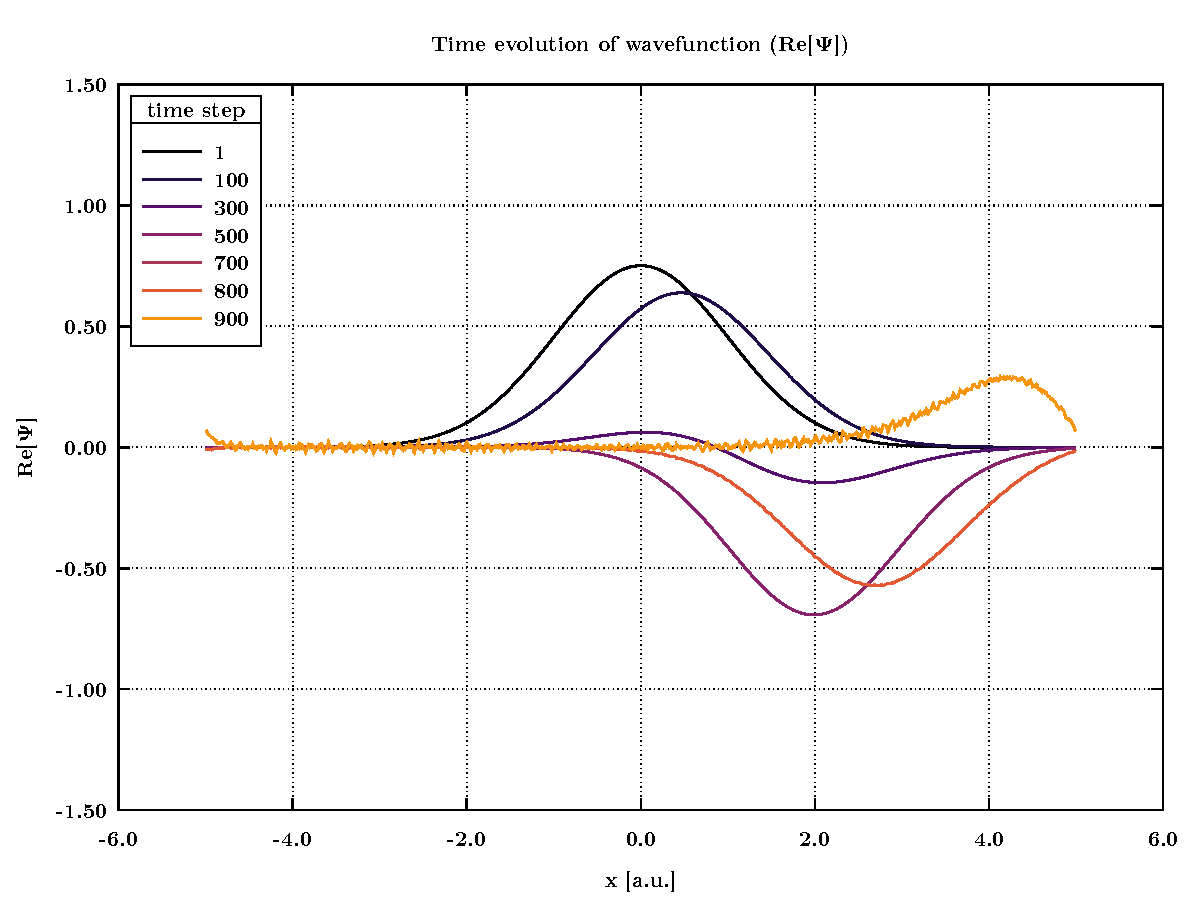
\includegraphics[width=1\textwidth]{image/state_re.pdf}
\end{minipage}
\begin{minipage}[]{0.48\linewidth}
\centering
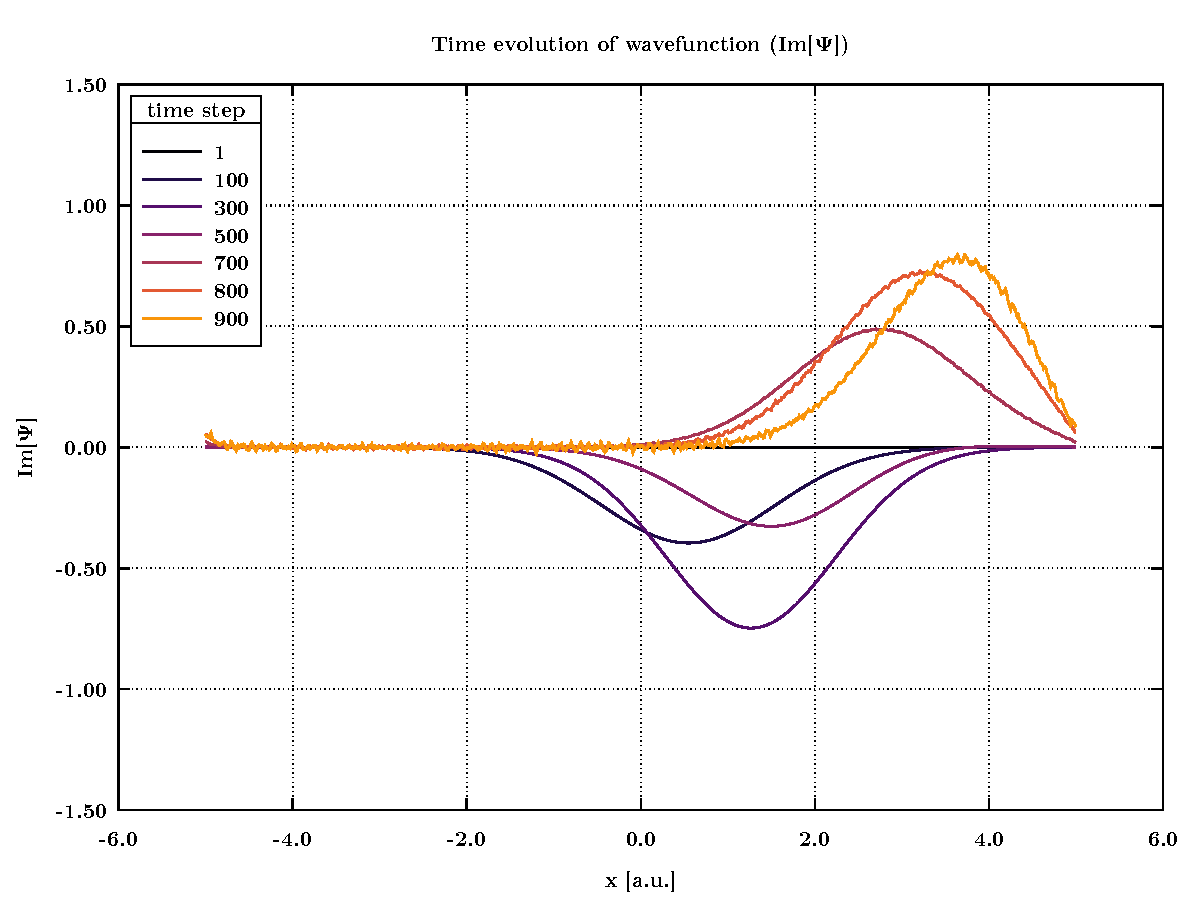
\includegraphics[width=1\textwidth]{image/state_im.pdf}
\end{minipage}
\caption{\label{fig:result_state} Plot of real and imaginary part of wave function \( \psi(x,t) \) at different time steps.}
\end{figure}

\begin{figure}[h!]
\centering
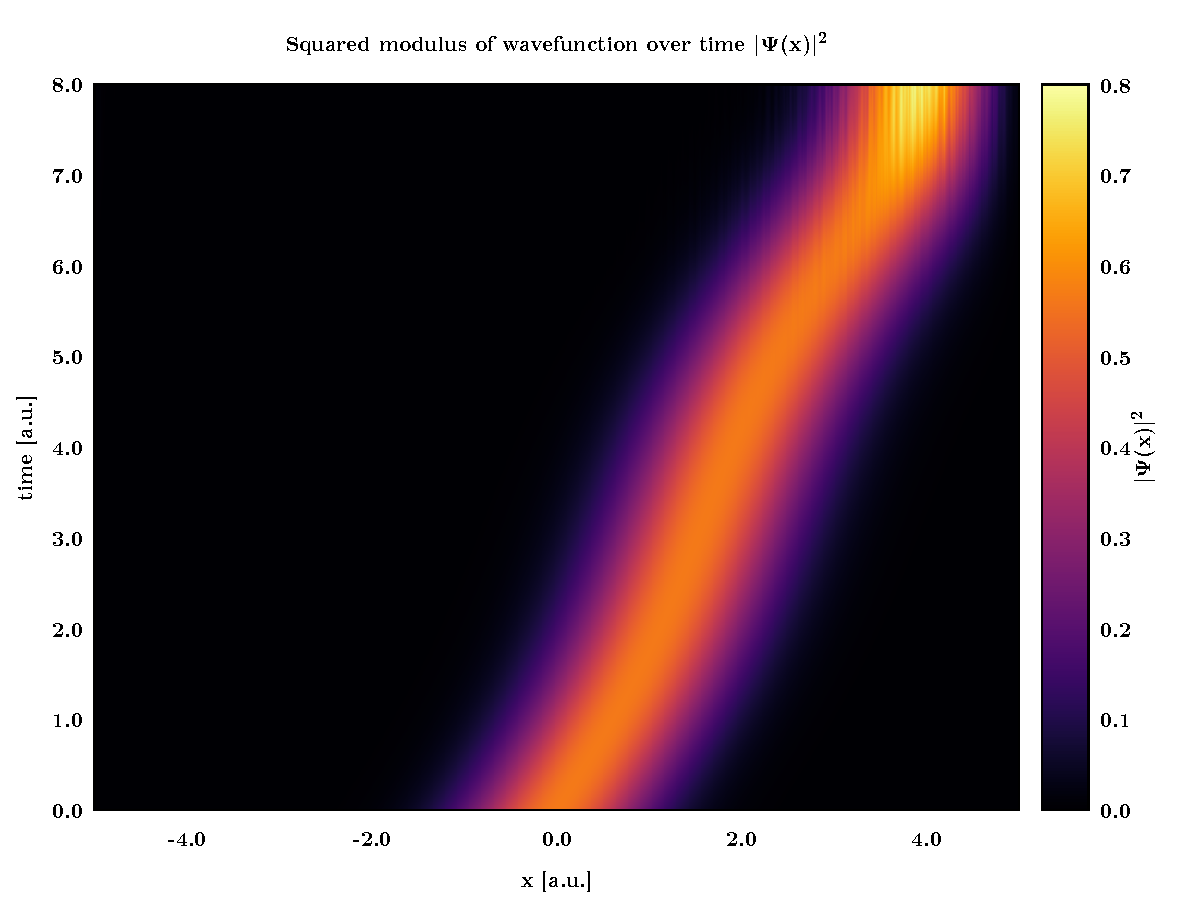
\includegraphics[width=0.5\textwidth]{image/color_map.pdf}
\caption{\label{fig:result_cmap} Colormap of square modulus of wave function over time. We note that the most probable position moves linearly in time with a slight oscillation component. Near to \( x=5 \) we have a non physical behavior associated to boundary effects.}
\end{figure}




\section{Self-evaluation}
By using the split operator method we can compute in an efficient way the time evolution of a wavefunction for a quantum harmonic oscillator. The implemented algorithm is fast and gives correct results. In a further development of the code, it could be interesting to study the behavior by changing the angular frequency \( \omega  \) parameter. Moreover, it could be interesting to apply split operator method to study other kind of quantum systems with kinetic ang potential operator which commute (to exploit the FFT algorithm).









\end{document}
